
%(BEGIN_QUESTION)
% Copyright 2006, Tony R. Kuphaldt, released under the Creative Commons Attribution License (v 1.0)
% This means you may do almost anything with this work of mine, so long as you give me proper credit

A pressure gauge is supposed to accurately indicate applied pressure over its full calibrated range.  In this example, a gauge with a range of 0 to 500 PSI is subjected to five different pressures along that range, and its response is accurate at all those points:

$$\includegraphics[width=15.5cm]{i00174x01.eps}$$

Describe, by drawing a set of five meter readings such as the set shown above, how a pressure gauge accurate at 0\% and 100\% of applied pressure -- but with a {\it nonlinearity} problem between the LRV and URV points -- might respond to the same five applied pressures.

\vskip 10pt

Furthermore, describe how a bourdon tube pressure gauge instrument might be adjusted for linearity.  In other words, how may a nonlinear pressure gauge be calibrated to become more linear? 

\vskip 20pt \vbox{\hrule \hbox{\strut \vrule{} {\bf Suggestions for Socratic discussion} \vrule} \hrule}

\begin{itemize}
\item{} Explain how keeping both ``As-Found'' and ``As-Left'' calibration records on instruments such as this pressure gauge make it possible to track long-term calibration drift.
\item{} Can a non-linearity error be corrected by adjusting the zero and/or span screws on an instrument?  Why or why not?
\end{itemize}

\underbar{file i00174}
%(END_QUESTION)





%(BEGIN_ANSWER)

Here is one example of how a pressure gauge might respond in a non-linear fashion to the same five applied pressures, while still being accurate at the LRV and URV points:

$$\includegraphics[width=15.5cm]{i00174x02.eps}$$

Here, the gauge reads high at the 25\% point (125 PSI), slightly low at the 50\% point (250 PSI), and low at the 75\% point (375 PSI), while still accurate at 0\% (0 PSI) and 100\% (500 PSI).

\vskip 10pt

Any adjustment that affects the {\it traveling angle} of the mechanism will have an effect on linearity.  Some (high-quality) pressure gauge mechanisms are equipped with an adjustable-length link to facilitate changes to this angle:

$$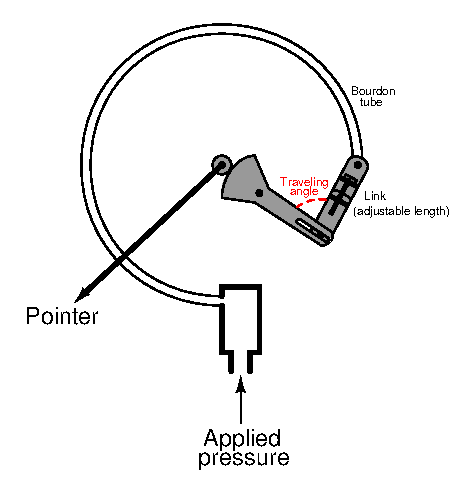
\includegraphics[width=15.5cm]{i00174x03.eps}$$

It is sage advice to {\it leave all angle adjustment(s) untouched} until all possible zero and span adjustments have been made to the instrument.  Usually, it is possible to get a nonlinear instrument to read within specified tolerance in a 5-point calibration just by adjusting the zero and span adjustments.

In many mechanical instruments, a simple linearity alignment is to apply a 50\% input signal and check for link/lever perpendicularity (that all links and levers intersect at 90$^{o}$ angles to each other).

%(END_ANSWER)





%(BEGIN_NOTES)

It should be noted that instrument nonlinearity does not imply an alternation between high and low error.  Fundamentally, nonlinearity is defined as {\it any} condition where the instrument reads accurately at (at least) two points, but not at all points along its calibrated range.

If the gauge were perfectly linear, accuracy at two points along its range would necessitate accuracy at {\it all} points along its range.  In reality, every instrument is nonlinear to some degree: the question is, how nonlinear can it be and still meet the minimum requirements for total accuracy?

\vskip 10pt

A practical application of {\it intentional} non-linearity in a link/lever system is the Ackerman angle in car steering systems.  You may wish to illustrate this for your students to help them understand the influence of the traveling angle in a mechanical gauge.

%INDEX% Measurement, pressure: nonlinearity in pressure gauge

%(END_NOTES)


